% Section content template for individual Educative lessons
% This file contains the actual content for a specific section
% Generated from Educative API section content

% Section: Activity Diagram for the Airline Management System
% Section ID: 5273648345907200
% Section Slug: activity-diagram-for-the-airline-management-system
% Generated: 2025-12-14T13:18:02.998181

Activity diagrams are an effective way to visualize the flow of messages from one activity to another within the system. There can be different activity diagrams that we can create for the airline management system. In this lesson, we will create activity diagrams for the following two activities:

\begin{itemize}
\item
\protect\phantomsection\label{z-MopNIQo7zNFhCQelSUX}
Creating an itinerary.
\item
\protect\phantomsection\label{_d3fg_K8mcb5FpjWwVFo8}
\textbf{Activity challenge:~} The user receives a confirmation notification after payment.
\end{itemize}

\subsection{Create an itinerary}\label{hefj461oJKz3o6fSDmBLG}
\\
The states and actions involved in this activity diagram are provided below.

\subsubsection{States}\label{SAPO2CXwtGjwzILBjqcbw}
\\
\textbf{Initial state:~} The customer chooses an option to create the itinerary.
\\
\textbf{Final state:}~A customer books their ticket.

\subsubsection{Actions}\label{Li4F24WQKnXe1jl5em2wP}
\\
The customer selects an option to create an itinerary online or through the front desk officer. The customer then selects their flights. Finally, the customer books their ticket.

\begin{figure}[htbp]
 \centering
 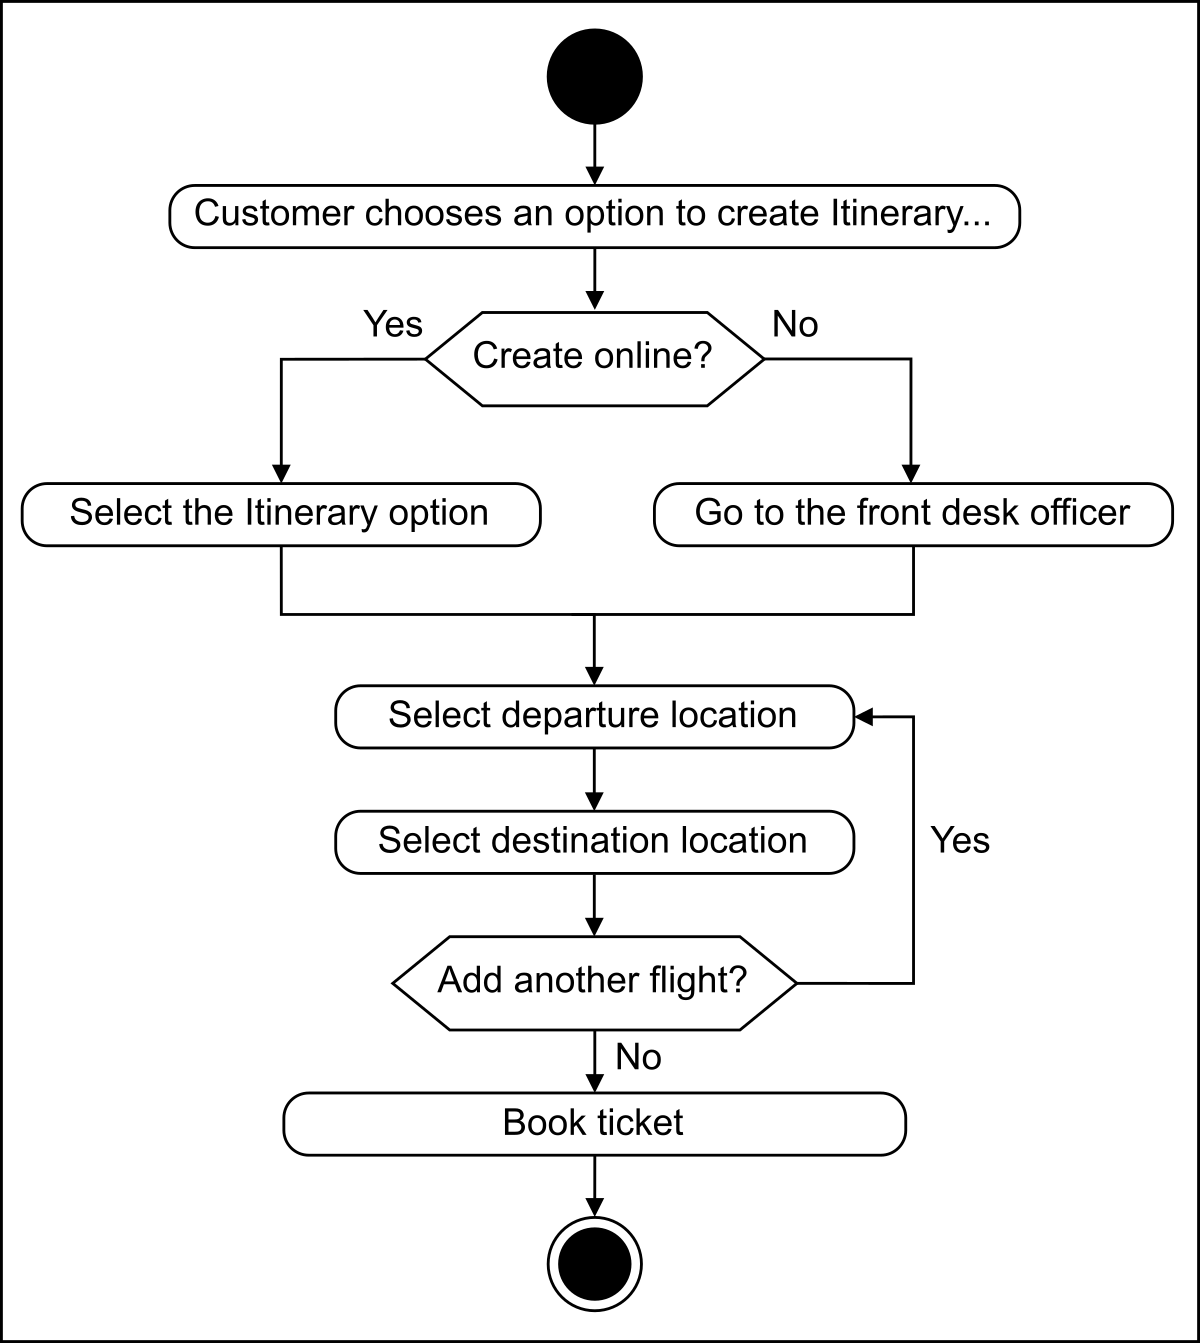
\includegraphics[width=0.5\textwidth]{Images/chapter_25/section_5273648345907200/5313243070595072.png}
 \caption{The activity diagram to create an itinerary}
\end{figure}

\subsection{Activity challenge: The user receives a confirmation notification after payment}\label{syvcAAl87sGAthCECq0g-}
\\
Let's create an activity diagram of a user receiving a confirmation notification after making the payment. A skeleton of the activity diagram is given below:

\begin{figure}[htbp]
 \centering
 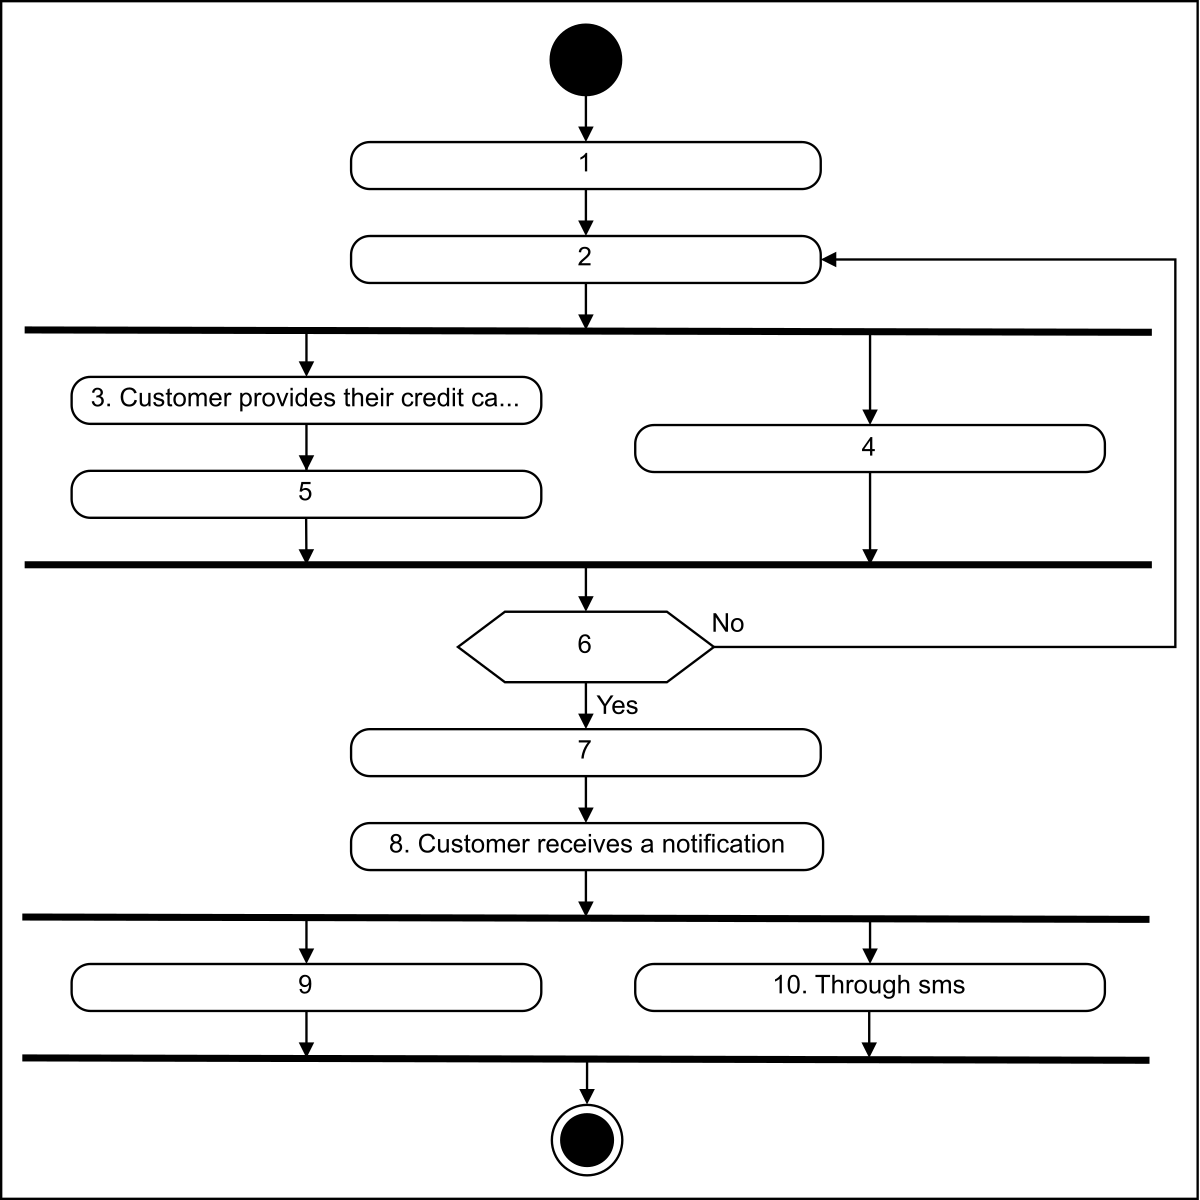
\includegraphics[width=0.5\textwidth]{Images/chapter_25/section_5273648345907200/5550210878275584.png}
 \caption{The activity diagram for a user receiving a confirmation notification after the payment}
\end{figure}

Notice that the actions in the diagram above are numbered from 1 to 10. The slots below represent the activities, and the arrows indicate the flow from one activity to another. Can you rearrange the slots below in the correct order they should appear in the activity diagram given above?
\begin{quote}
\textbf{Note:~} If you're stuck, click the ``Show Solution'' button.
\end{quote}

Alternatively, click the ``Show complete diagram'' button below to see the complete activity diagram.

We've looked at some of the activity diagrams of the airline management system.~In the next lesson, we'll present the code for our designed classes in some of the most popular languages.

% End of section content